\chapter{$k$-Median with outliers}
\label{cap:kmedout}
The second problem addressed is the $k$-median with outliers. Its definition is recalled, and then a $7.081(1 + \eps)$-approximation that runs in time $n^{O(1/\eps^2)}$, due to Krishnaswamy, Li, and Sandeep~\cite{KLS2018} is presented. We refer to this algorithm as the KLS approximation.

\begin{problem}[$k$-Median with outliers]
Given a metric space $(F \cup D,d)$, where $F$ is a set of facility locations, $D$ is a set of clients, and $d : (D \cup F) \times (D \cup F) \to \mathbb{R}_+$ is a metric, an integer $k$ representing the number of facility locations that can be opened and an integer $m$ representing the coverage requirement, the goal is to find a set $S \subseteq F$ and a set $C \subseteq D$ such that $|S| \le k$ and $|C| \geq m$, and $S$ and $C$ minimize $\sum_{j \in C} d(j,S)$.
We assume that there are no colocated facilities. Since the facilities have no capacities, colocated facilities are redundant. However, clients are allowed to be colocated with each other or with a facility.
\end{problem}

The starting point of the KLS approximation is the natural LP relaxation for the problem. One of the main contributions of~\cite{KLS2018} is an iterative algorithm which can round the natural LP to compute an almost-integral solution, with at most two fractional variables. Unfortunately, the integrality gap between almost-integral solutions and fully-integral ones is unbounded. Thus, the KLS approximation uses sparsification techniques as a preprocessing step to overcome this gap.

In the preprocessing step, some facilities are chosen to be pre-opened. Based on that, the notion of \emph{extended instances} is defined.

\begin{definition}
An \emph{extended instance} of the $k$-median with outliers problem is denoted by a tuple $(F, D, d, k, m, S_0)$, where $(F, D, d, k, m)$ is an instance of the $k$-median with outliers problem, and $S_0 \subseteq F$ is a set of \emph{pre-opened} facilities. A feasible solution for an extended instance is a pair $(S, C)$, where $S \subseteq F$ is a set of facilities such that $|S| \leq k$ and $S_0 \subseteq S$, and $C \subseteq D$ is a set of clients such that $|C| \geq m$.
\end{definition}

\subsection{The natural LP and integrality gaps}
In this section, we present the natural LP relaxation of the $k$-median with outliers problem and two different gap examples that illustrate distinct reasons why the integrality gap arises. For an instance $(F,D,d,k,m)$ of the $k$-median with outliers problem, we define the following LP:

\begin{equation}\tag{$\text{LP}_{\text{basic}}$} \label{LP-basic} 
\begin{aligned} 
\text{Minimize} \quad &\sum_{i \in F} \sum_{j \in D} x_{ij} \,d(i,j) \\
\text{subject to} \quad &\sum_{i \in F} y_i \le k, \\ 
&x_{ij} \le y_i, && \forall i \in F, \ j \in D,\\ 
&\sum_{i \in F} x_{ij} \le 1, && \forall j \in D,\\ 
&\sum_{j \in D} \sum_{i \in F} x_{ij} \ge m, \\ 
&x \in[0,1]^{F\times D}, \\
&y \in [0,1]^F.
\end{aligned} 
\end{equation}

Here, the variable $y_i$ indicates how much the facility $i \in F$ is (fractionally) open, while $x_{ij}$ indicates how much the client $j \in D$ is fractionally served by facility $i$. Note that the feasible solutions for this program represent fractionally open facilities that fractionally cover clients, satisfying the coverage constraints and bounding the number of fractionally opened facilities. Once the $y$-values are fixed, the optimal choice for the $x$-variables can be determined by a simple greedy allocation.

The unbounded integrality gap essentially arises when we try to round a fractional solution into a fully-integral one. To build intuition, suppose we are able to round the LP solution into an almost-integral solution, where only two facilities, say $i_1$ and $i_2$, have strictly fractional values $y_1 = 1-\rho$ and $y_2 = \rho$ for some $\rho > 0$. To obtain a fully-integral solution while maintaining the number $m$ of served clients, a natural approach is to increase one of $y_1$ or $y_2$ to $1$ and decrease the other one to $0$. However, each of these two operations incurs a specific cost that can be unbounded compared to the LP cost. This is illustrated by the following two gap examples.

\paragraph{Gap Example 1 (Cost of increasing a fractional facility).}
Consider the instance illustrated in Figure~\ref{fig:gap_examples}(a), which contains two clusters separated by a large distance. In the first cluster, there is a facility $i_1$ colocated with $t^3$ clients. In the second cluster, there is a facility $i_2$ at distance $1$ from $t^3 + t^2$ clients. Let $k = 1$ and $m = t^3 + t$. An integral optimal solution is forced to open $i_2$, incurring a cost of $m = t^3 + t$. However, a fractional LP solution can open a $1-1/t$ fraction of $i_1$ and a $1/t$ fraction of $i_2$. This solution serves $(1-1/t)t^3 + (1/t)(t^3+t^2) = t^3 + t = m$ clients. The cost of this LP solution is exactly the fractional connection to $i_2$, which is $(1/t) \times (t^3+t^2) = t^2+t$. The integrality gap is $\frac{t^3+t}{t^2+t}$, which grows unbounded as $t$ increases. This gap arises because the cost of fully connecting the clients to the facility that was increased to $1$ (facility~$i_2$) explodes.

\paragraph{Gap Example 2 (Cost of decreasing a fractional facility).}
Consider the instance illustrated in Figure~\ref{fig:gap_examples}(b), with three facilities $i_0$, $i_1$, and $i_2$. Facilities $i_0$ and $i_1$ are colocated with $2t$ clients each, and $d(i_0, i_1) = 1$. Facility $i_2$ is located far away and is colocated with $t$ clients. Let $k = 2$ and $m = 4t + 1$. An integral solution opens $i_0$ and $i_2$, serves the $3t$ clients colocated at these facilities (at zero cost), and serves $t+1$ clients from $i_1$ to $i_0$, incurring a total cost of $t+1$. On the other hand, an LP solution can set $y_0 = 1$, $y_1 = 1-1/t$, and $y_2 = 1/t$. It fully serves the $4t$ clients at $i_0$ and $i_1$, each client at $i_1$ is served by $i_1$ to an extent of $1 - 1/t$ and served by $i_0$ to an extent of $1/t$, and serves each client at $i_2$ to an extent of $1/t$, covering exactly $2t + 2t(1- 1/t + 1/t)+ t(1/t) = 4t+1 = m$ clients. Since each client at $i_1$ is served by $i_0$ to an extent of $1/t$, the LP cost is $2t \times (1/t) = 2$. The integrality gap is $\frac{t+1}{2}$, which is also unbounded. This gap arises because decreasing $y_1$ to $0$ forces many clients to be reassigned, and this relocation cost can be arbitrarily large.


\begin{figure}[h]
    \centering
    \resizebox{\textwidth}{!}{
    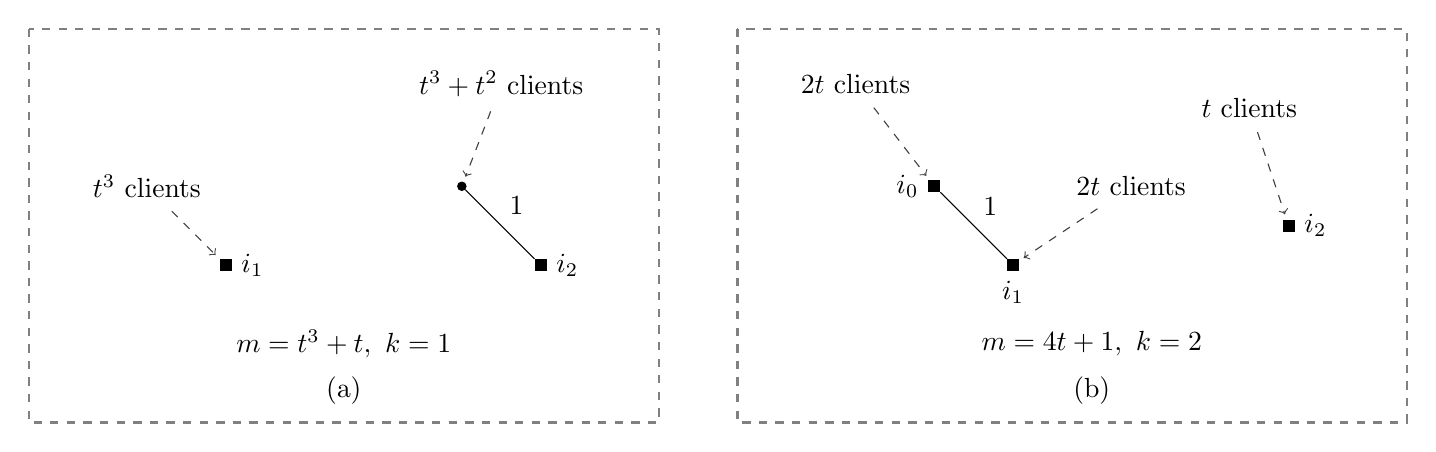
\begin{tikzpicture}[
    facility/.style={rectangle, draw, fill=black, inner sep=0pt, minimum size=4pt},
    client/.style={circle, draw, fill=black, inner sep=0pt, minimum size=3pt},
    pointer/.style={->, dashed, shorten >=2pt, shorten <=2pt, color=darkgray}
]

% Gap Example 1
\begin{scope}
    \draw[dashed, gray, thick] (-2.5, 2.5) rectangle (5.5, -2.5);

    \node[facility, label=right:$i_1$] (i1) at (0, -0.5) {};
    \node[client] (c2) at (3, 0.5) {};
    \node[facility, label=right:$i_2$] (i2) at (4, -0.5) {};

    \draw (c2) -- node[above right] {$1$} (i2);

    \node (t1) at (-1, 0.5) {$t^3$ clients};
    \draw[pointer] (t1) -- (i1);

    \node (t2) at (3.5, 1.8) {$t^3 + t^2$ clients};
    \draw[pointer] (t2) -- (c2);

    \node at (1.5, -1.5) {$m = t^3 + t,\ k = 1$};
    \node at (1.5, -2.1) {(a)};
\end{scope}

% Gap Example 2
\begin{scope}[shift={(9, 0)}]
    
    \draw[dashed, gray, thick] (-2.5, 2.5) rectangle (6, -2.5);

    \node[facility, label=left:$i_0$] (i0) at (0, 0.5) {};
    \node[facility, label=below:$i_1$] (i1) at (1, -0.5) {};
    \node[facility, label=right:$i_2$] (i2) at (4.5, 0) {};

    \draw (i0) -- node[above right] {$1$} (i1);

    \node (t3) at (-1, 1.8) {$2t$ clients};
    \draw[pointer] (t3) -- (i0);

    \node (t4) at (2.5, 0.5) {$2t$ clients};
    \draw[pointer] (t4) -- (i1);

    \node (t5) at (4, 1.5) {$t$ clients};
    \draw[pointer] (t5) -- (i2);


    \node at (2, -1.5) {$m = 4t + 1,\ k = 2$};
    \node at (2, -2.1) {(b)};
\end{scope}

\end{tikzpicture}}
    \caption{Two gap instances illustrating the cost of increasing and decreasing fractional facilities.}
    \label{fig:gap_examples}
\end{figure}


\subsection{Preprocessing the instance}
To handle the first type of bad instances, where the cost of increasing a fractional facility to $1$ is unbounded (as seen in Figure~\ref{fig:gap_examples}(a)), it is necessary to bound the connection cost of clients fractionally connected to a facility. This cost is often referred to as the \emph{star cost} of the facility.
Notice that, in an optimal solution, the star cost of any facility is at most the optimal cost.
Thus, if we know an upper bound $U$ on the optimal cost, we can force the linear programming relaxation to avoid solutions with star costs greater than this upper bound by adding a constraint that bounds the star cost of every facility $i \in F$ to be at most $y_i U$. In fact, one can reduce the additional cost, incurred by integrally opening a fractional facility, to a small fraction $\rho U$, for some small constant $\rho > 0$ that goes to $0$ as $\epsilon$ goes to $0$.
Fix an optimal solution.
One can guess the set of facilities in this optimal solution whose star costs exceeds $\rho U$ and pre-open them. Since the total optimal cost is bounded by $U$, there can be at most $1/\rho$ such facilities. This motivates the use of a set $S_0$ of pre-opened facilities introduced in the definition of extended instances. By pre-opening these expensive facilities, we can add a constraint in~\eqref{LP-basic} for all the remaining non-pre-opened facilities $i \in F \setminus S_0$,
\[
\sum_{j \in D} x_{ij} \, d(i,j) \le y_i \cdot \rho U.
\]
By doing that, an optimal solution remains a feasible solution for~\eqref{LP-basic} augmented with this new constraint, since the facilities that violate it are already fully opened in~$S_0$.

To handle the second type of bad instances, where the cost of decreasing a fractional facility to $0$ is unbounded (as seen in Figure~\ref{fig:gap_examples}(b)), it is necessary to bound the reassignment cost of the clients.
Notice that, in any optimal solution with total cost at most $U$, the number of clients paying a connection cost of at least $L > 0$ is at most $U/L$. Thus, if we know an upper bound $U$ on the optimal cost, we can force the linear programming relaxation to avoid solutions where many clients incur a high connection cost when reassigned to another open facility.
To do this, we restrict the connection distances locally. As we will formalize later, it is possible to compute a vector of radius $(R_j)_{j \in D}$ satisfying two key properties: (i) for any $L > 0$ and some constant $\delta$, the number of clients $j$ in any ball of radius $\delta L$ such that $R_j$ is greater than some $\Theta(L)$ is at most $O(1)U/L$, where $O(1)$ is a constant that depends on the value of $\delta$, and (ii) there exists a feasible solution of cost $O(1)U$ that respects these bounds. Using these radius, we add a constraint on the allowed connections to~\eqref{LP-basic}:
\[
x_{ij} = 0 \quad \text{for all } i \in F \text{ and } j \in D \text{ such that } d(i,j) > R_j.
\]
By doing that, one ensures that the cost of reassigning clients remains controlled.
However, while these properties prevent the cost from exploding, they only guarantee a constant factor approximation. To reduce the additive error further, we need the third preprocessing idea.

The previous preprocessing idea bounds the reassignment cost, but only guarantee a feasible solution of cost $O(1)\OPT$, where $\OPT$ is the cost of an optimal solution. To try to reduce this additive factor to a small constant $\eps$, suppose that, in the optimal solution, the number of clients in any ball of radius $\delta L$ with connection cost at least $L$ is at most $\rho \OPT/L$, for some small $0 \leq \rho < 1$. One can bound by $O(\rho)\OPT$ the total increase in cost of reassigning these clients when shutting down one facility. We call this kind of instance \emph{sparse}, and the third preprocessing idea consists of guessing \emph{dense regions} (that will be defined later) so that the remaining instance is sparse.

Let $(S^*, C^*)$ be an optimal solution to an extended instance $I' = (F, D, d, k, m, S_0)$ with cost at most $U$. For each facility $i \in S^*$, let $C_i^*$ be the set of clients in $C^*$ that have $i$ as their closest open facility. We assume that each $j \in C^*$ is in exactly one $C_i^*$ for some $i \in S^*$. We guarantee this by breaking ties arbitrarily.

\begin{definition}[Sparse Extended Instances]
    \label{def:sparse_extended_instances}
Given an extended instance ${I' = (F,D,d,k,m,S_0)}$, parameters $\rho, \delta \in (0, 1/2)$, and $U \ge 0$. Let $(S^*, C^*)$ be a feasible solution to $I'$ with cost at most $U$. We say that $I'$ is $(\rho, \delta, U)$-sparse w.r.t.\ $(S^*, C^*)$ if:
\begin{enumerate}[label=\thedefinition\alph*)]
    \item \label{def:sparse_extended_instances_a} for every $i \in S^* \setminus S_0$, one has $\sum_{j \in C_i^*} d(j, i) \leq \rho U$;
    \item \label{def:sparse_extended_instances_b} for every $p \in F \cup D$, one has $|\mathcal{B}(p, \delta \cdot d(p, S^*)) \cap C^*| \cdot d(p, S^*) \leq \rho U$.
\end{enumerate}
\end{definition}

In sparse extended instances, both the star cost of non-pre-opened facilities and the total connection cost of clients in small neighborhoods are strictly bounded by $\rho U$.

Given an instance $I = (F,D,d,k,m)$ of the $k$-median problem with outliers, the authors of~\cite{KLS2018} describe a procedure to generate a set of instances such that one of them is a sparse extended instance with a bonus property. It is stated in the following theorem and we will briefly describe the procedure.

\begin{theorem}[Theorem 3.2 in~\cite{KLS2018}] \label{thm:sparsification}
Suppose we are given an instance $I = (F, D, d, k, m)$, parameters $\rho, \delta \in (0, 1/2)$, and an upper bound $U$ on the cost of an optimal solution $(S^*, C^*)$ to $I$ (which is not given to us). There is an $n^{O(1/\rho)}$-time algorithm that outputs $n^{O(1/\rho)}$ extended instances such that one of them, say $I'$, has the form $(F, {D' \subseteq D}, d, k,{ m' = |C^* \cap D'|}, S_0 \subseteq S^*)$ and satisfies:
\begin{enumerate}[label=\thedefinition\alph*)]
    \item \label{thm:sparsification_a} $I'$ is $(\rho, \delta, U)$-sparse w.r.t.\ the solution $(S^*, C^* \cap D')$;
    \item \label{thm:sparsification_b} $\frac{1-\delta}{1+\delta} \sum_{j \in C^* \setminus D'} d(j, S_0) + \sum_{j \in C^* \cap D'} d(j, S^*) \leq U$.
\end{enumerate}
\end{theorem}
Property~\ref{thm:sparsification_b} means that the cost of the solution $(S^*, C^* \cap D')$ for the residual sparse instance $I'$ combined with the approximate cost of reconnecting the excluded clients $C^* \setminus D'$ to the pre-opened facilities $S_0$, remains upper bounded by $U$. 

The idea is that we need to add to $S_0$ a constant number, parametrized by $\rho$, of facilities to ensure~\ref{def:sparse_extended_instances_a} and remove a constant number of balls to ensure~\ref{def:sparse_extended_instances_b}. It takes $O(n)$ to guess one facility to be removed, and $O(n^3)$ to guess a ball, since we need to guess the point which the ball is centered, and to guess the radius, we choose one of the $O(n^2)$ distances of the metric. We simply brute force every possibility, returning an instance for each of them. One of the instances will satisfy the properties of the theorem. The proof consists of showing how to obtain the desired instance if we know an optimal solution.

\begin{proof}
    First, assume that we know an optimal solution $(S^*,C^*)$ of the instance $I = (F,D,d,k,m)$. Also, let $\rho,\delta$ and $U$ be parameters as defined in the theorem. Also, for each $i \in S^*$, let $C_i^* \subseteq C^*$ be the set of clients of $C^*$ such that $i$ is the closest facility of~$S^*$. We assume that each $j \in C^*$ is in exactly in one $C_i^*$, by breaking the ties arbitrarily. We will iteratively choose a facility from $S^*$ that violates~\ref{def:sparse_extended_instances_a} and add it to $S_0$, until it holds. Then, we will iteratively choose a point that violates~\ref{def:sparse_extended_instances_b}, add it to $S_0$ and remove the respective ball, until the property holds. We start with $D' \coloneqq D$ and $S_0 \coloneqq \emptyset$ and will stop with a $(\rho,\delta,U)$-sparse w.r.t $(S^*,C^* \cap D')$ instance $I' = (F,D',d,k,m' = |C^* \cap D'|,S_0)$.

    To guarantee property~\ref{def:sparse_extended_instances_a} we add to $S_0$ the set of faciltiies $i \in S^*$ such that $\sum_{j \in C_i^*} d(j, i) > \rho U$. There are at most $1/\rho$ such facilities. After this, we have that $\sum_{j \in C_i^* \cap D'} d(j,i) \leq \sum_{j \in C_i^*} d(j, i) \leq \rho U$.

    To guarantee property~\ref{def:sparse_extended_instances_b}, while there exists $p \in F \cup D$ such that
    \[
    |\mathcal{B}(p, \delta \cdot d(p, S^*)) \cap C^* \cap D'| \cdot d(p, S^*) > \rho U,
    \]
    we add in $S_0$ the facility $i \in S^*$ which is nearest from $p$, and update ${D' \gets D' \setminus \mathcal{B}(p, \delta \cdot d(p,S^*))}$. By triangle inequality, every client $j$ removed at this step satisfies $d(j,S^*) \ge d(p,S^*) - d(j,p) \ge (1-\delta)\, d(p,S^*)$, and also
    \[
    d(j,S_0) \le d(j,i) \le d(j,p) + d(p,i) \le \delta\, d(p,S^*) + d(p,S^*) \le \frac{1+\delta}{1-\delta}\, d(j,S^*).
    \]
    Moreover, since every removed client $j$ satisfies $d(j,S^*) \ge (1-\delta)d(p,S^*)$, the total cost contributed by the clients removed at this step is at least
    \[
    |\mathcal{B}(p,\delta \cdot d(p,S^*)) \cap C^* \cap D'| \cdot (1-\delta)\, d(p,S^*) > (1-\delta)\rho U,
    \]
    where the last inequality follows from the violated condition. Since the total cost of $(S^*,C^*)$ is at most $U$, and each iteration removes clients whose combined cost exceeds $(1-\delta)\rho U$, this procedure runs for at most $\frac{1}{\rho(1-\delta)} = O(1/\rho)$ iterations before it terminates. When it stops, we have $|\mathcal{B}(p,\delta\cdot d(p,S^*)) \cap C^* \cap D'|\cdot d(p,S^*) \le \rho U$ for every $p\in F\cup D$, so Property~\ref{def:sparse_extended_instances_b} holds, and the resulting instance is $(\rho, \delta, U)$-sparse w.r.t. the solution $(S^*,C^*\cap D')$.

    It remains to check Property~\ref{thm:sparsification_b}. Every client $j$ removed from $D'$ during the second phase, i.e., every $j \in C^*\setminus D'$, satisfies $\frac{1-\delta}{1+\delta}d(j,S_0) \le d(j,S^*)$, by the bound established above. Summing this inequality over all such clients and adding $\sum_{j\in C^*\cap D'} d(j,S^*)$ to both sides gives
    \[
    \frac{1-\delta}{1+\delta}\sum_{j\in C^*\setminus D'} d(j,S_0) + \sum_{j\in C^*\cap D'} d(j,S^*) \le \sum_{j\in C^*\setminus D'} d(j,S^*) + \sum_{j\in C^*\cap D'} d(j,S^*) = \sum_{j\in C^*} d(j,S^*) \le U,
    \]
    which is exactly Property~\ref{thm:sparsification_b}.

    This finishes the construction assuming the optimal solution $(S^*,C^*)$ is known. Since we do not have access to it in practice, we cannot run this procedure directly. However, as discussed above, the construction only ever adds $O(1/\rho)$ facilities to $S_0$ and removes $O(1/\rho)$ balls of clients from $D'$, and each ball is determined by its center $p$ and its radius $\delta \cdot d(p,S^*)$, which is one of the $O(n^2)$ pairwise distances of the metric. Thus, there are at most $n^{O(1/\rho)}$ possible instances $(F,D',d,k,m',S_0)$ that could arise from this procedure. We simply enumerate all of them; one of these instances is guaranteed to be the one produced by running this procedure that knows an optimal solution $(S^*,C^*)$, which satisfies Properties~\ref{thm:sparsification_a} and~\ref{thm:sparsification_b}.
\end{proof}

The concept of sparse instances is utilized to construct the vector $(R_j)_{j \in D}$ representing the maximum connection cost for each client. Once these bounds are found, the notion of sparsity is no longer required for the subsequent steps of the algorithm. In the following theorem, we state the properties of the values $R_j$ that can be efficiently computed, followed by a brief description of the procedure for their construction.

\begin{theorem}[Theorem 3.3 in~\cite{KLS2018}] \label{thm:radius_existence}
Let $I' = (F, D', d, k, m, S_0)$ be a $(\rho, \delta, U)$-sparse instance w.r.t. some solution $(S^*, C^*)$ of $I'$, for some $\rho, \delta \in (0, 1/2)$ and $U \ge 0$. Let $U' \le U$ be the cost of $(S^*, C^*)$ to $I'$. Then, given $I', \rho, \delta, U$, we can efficiently find a vector $(R_j)_{j \in D'} \in \mathbb{R}^{D'}_{\ge 0}$ such that:
\begin{enumerate}
    \item for every $t > 0$ and $p \in F \cup D'$, we have:
    \[ \left| \left\{ j \in \mathcal{B} \left( p, \frac{\delta t}{4 + 3\delta} \right) \cap D' : R_j \ge t \right\} \right| \le \frac{\rho(1 + 3\delta/4)}{(1 - \delta/4)} \cdot \frac{U}{t}; \]
    \item there exists a solution to $I'$ of cost at most $(1 + \delta/2)U'$ where if $j$ is connected to $i$ then $d(i, j) \le R_j$; moreover, the total cost of clients connected to any facility $i \notin S_0$ in this solution is at most $\rho (1 + \delta/2) U$.
\end{enumerate}
\end{theorem}

The first property states that, in a ball of radius $\Theta(t)$, the number of clients $j$ with $R_j \ge t$ is $O(\rho) \cdot U/t$. The first part of the second property guarantees that there exists a near-optimal solution respecting these upper bounds $R_j$ on the connection distances for all clients $j$, while the second part ensures that the star costs for facilities in $F \setminus S_0$ remain bounded in this solution.

Krishnaswamy \emph{et al.} prove this theorem by providing such an algorithm. Their algorithm first finds a vector $(\hat{R}_j)_{j \in D'}$ such that
\begin{itemize}
    \item[(i)] for every $t > 0$ and $p \in F \cup D'$, we have:
    \begin{equation}
        \label{ineq:Rhat}
        \left| \left\{ j \in \mathcal{B} \left( p, \frac{\delta t}{4} \right) \cap D' : \hat{R}_j \ge t \right\} \right| \le \frac{\rho}{1 - \delta/4} \cdot \frac{U}{t};
    \end{equation}
    \item[(ii)] there exists a solution to $I'$ of cost at most $(1 + \delta/2)U'$ where if $j$ is connected to~$i$ then $d(i, j) \le (1+3\delta/4)\hat{R}_j$; moreover, the total cost of clients connected to any facility $i \notin S_0$ in this solution is at most $\rho (1 + \delta/2) U$.
\end{itemize}
Then, they set $R_j \gets \hat{R}_j (1+3\delta/4)$ for all $j \in D'$.

\begin{algorithm}
\caption{Construct $\hat{R}$} \label{alg:construct_R}
\begin{algorithmic}[1]
    \For{each $j \in D'$}
    \State $\hat{R}_j \gets 0$
    \EndFor
    \For{each $t' \in \{d(i,j) : i \in F, j \in D'\} \setminus \{0\}$ in decreasing order}
    \For{each $j' \in D'$ such that $\hat{R}_{j'} = 0$}
    \If{ letting $\hat{R}_{j'} = t'$ does not violate~\eqref{ineq:Rhat} for $t = t'$ and any $p \in F \cup D'$}
    \State $\hat{R}_{j'} \gets t'$
    \EndIf
    \EndFor
    \EndFor

\State \Return $\hat{R}$
\end{algorithmic}
\end{algorithm}

In the beginning of the procedure,~\eqref{ineq:Rhat} holds for all clients since $\hat{R}_j = 0$. The idea is that the procedure always maintains the inequality~\eqref{ineq:Rhat}, and this is sufficient to prove that (i) holds. 

To prove that property (ii) holds, the authors show such a solution. They construct a mapping $f : C^* \to D'$, and the set of clients that satisfies property (ii) is $f(C^*)$. They start by setting $f(j) \coloneqq j$, for $j \in C^*$, and then apply the following procedure. If a client $j \in C^*$ has a connection cost $c_j^* > (1 + 3\delta/4)\hat{R}_j$, then there is a nearby ball with many clients with $\hat{R}$ value at least $c_j^*$. Formally, they update $f(j)$ to be a client in $D' \setminus f(C^*)$ such that $d(f(j),j) \leq \delta c_j^*/2$ and $\hat{R}_{f(j)} \geq c_j^*$.
Suppose that $j$ is mapped to $i \in S^*$. Let us connect $f(j)$ to $i$. Note that $d(f(j),i) \leq d(f(j),j) + d(j,i) \leq (1 +\delta/2)c_j^*$. Thus, it is easy to see that property (ii) holds. The authors then use the fact that the instance is sparse to show that it is always possible to find an $f(j)$ that satisfies the updating inequalities and that this client is not already mapped in $f(C^*)$.



\subsection{The iterative rounding framework}
In this section we present the randomized algorithm used in the KLS approximation that receives an extended $k$-median with outliers instance, some parameters and the vector $R$ constructed by {Algorithm~\ref{alg:construct_R}}, and builds an approximate solution for this instance. 

The input of the algorithm is an instance $I = (F,D,d,k,m,S_0)$, parameters $\rho,\delta \in (0,1/2)$, $U \geq 0$ and a vector $R \in \mathbb{R}_{\geq 0}^{D}$. There is a parameter $U' \in [0,U]$ (which is not given to the algorithm) such that the properties of Theorem~\ref{thm:radius_existence} hold. 
The algorithm will output a solution to $I$ of cost at most $7.081(1 + \delta/2)U' + O(\rho/\delta)U$. The algorithm will have two phases: in the first phase, it uses an iterative rounding framework and obtain an almost-integral solution for $I$, with cost $7.081(1 + \delta/2)U'$; in the second phase, it converts the almost-integral solution to an integral one with an additional cost of $O(\rho/\delta)U$.

\subsubsection{The Strengthened LP}

To begin the first phase, we strengthen the basic LP relaxation~\eqref{LP-basic} by adding the constraints derived from the preprocessing steps. For notational convenience, let $\tilde{U} \coloneqq (1 + \delta/2)U$ and $\tilde{U}' \coloneqq (1 + \delta/2)U'$. The strengthened linear program, denoted by $\text{LP}_{\text{strong}}$, is formulated as follows:
\begin{align} \tag{$\text{LP}_{\text{strong}}$} \label{LP-strong}
\text{Minimize} \quad &\sum_{i \in F} \sum_{j \in D} x_{ij} d(i,j) \\
\text{subject to} \quad &\text{constraints of } \eqref{LP-basic}, \nonumber \\
& y_i = 1, \quad &&\forall i \in S_0, \nonumber \\
& x_{ij} = 0, \quad &&\forall i \in F, \ j \in D \text{ s.t. } d(i,j) > R_j, \nonumber \\
& \sum_{j \in D} x_{ij} d(i,j) \leq \rho \tilde{U} y_i, \quad &&\forall i \in F \setminus S_0, \nonumber \\
& x_{ij} = 0, \quad &&\forall i \in F \setminus S_0, \ j \in D \text{ s.t. } d(i,j) > \rho \tilde{U}. \nonumber
\end{align}

\begin{lemma}[Lemma 4.1 in~\cite{KLS2018}] \label{lem:strong_lp_cost}
The cost of an optimal solution to~\eqref{LP-strong} is at most $\tilde{U}' = (1 + \delta/2)U'$.
\end{lemma}

The lemma comes from the solution guaranteed by property 2 of Theorem~\ref{thm:radius_existence} which is a feasible solution to~\ref{LP-strong} with cost $\tilde{U}'$.

\subsubsection{Eliminating the $x$ variables}

As previously mentioned, once the values for the vector $y$ are fixed, optimal values for the $x$ variables can be determined via a simple greedy allocation. Based on this observation, our next step is to eliminate the variables $x_{ij}$ to construct an auxiliary LP that depends exclusively on the $y$ variables.

Suppose we have an optimal solution $(x,y)$ to~\eqref{LP-strong} such that, for all $i \in F$ and $j \in D$, either $x_{ij} = y_i$ or $x_{ij} = 0$. In this scenario, we could easily eliminate the $x$ variables and deal with an LP over the $y$ variables. To simulate this behavior, we apply a standard technique used in $k$-median algorithms: we split each fractional facility $y_i$ by creating collocated copies of the facilities in $F$. However, in our setting, we must be careful during this process to maintain the constraint $\sum_{j \in D} x_{ij}\, d(i,j) \leq \rho\, \tilde{U} y_i$ for each $ i \in F \setminus S_0$ of~\eqref{LP-strong}.

\begin{lemma}[Lemma 4.2 in~\cite{KLS2018}] \label{lem:eliminate_x}
By adding collocated facilities to $F$, we can efficiently obtain a vector $y^* \in [0,1]^F$ and a set of allowed facilities $F_j \subseteq \mathcal{B}(j, R_j) \cap F$ for every client $j \in D$, satisfying the following properties:
\begin{itemize}
    \item[(a)] For each client $j \in D$, we have $y^*(F_j) \leq 1$;
    \item[(b)] The total fractional opening of facilities satisfies $y^*(F) \leq k$;
    \item[(c)] The total fractional client coverage satisfies $\sum_{j \in D} y^*(F_j) \geq m$;
    \item[(d)] The bounded connection cost satisfies $\sum_{j \in D} \sum_{i \in F_j} y^*_i d(i, j) \leq \tilde{U}'$;
    \item[(e)] For each pre-opened facility $i \in S_0$, we have $\sum_{i' \text{ collocated with } i} y^*_{i'} = 1$;
    \item[(f)] For every facility $i$ that is not collocated with any facility in $S_0$, the star cost satisfies $\sum_{j \in D : i \in F_j} y^*_i d(i, j) \leq 2\rho\tilde{U}$.
\end{itemize}
\end{lemma}

The authors of~\cite{KLS2018} prove this lemma constructively by splitting the fractional facilities into collocated copies while building a set $F_j$ for each $j \in D$. First, take an solution $(x,y)$ for~\eqref{LP-strong}. For each facility $i \in F$ and client $j \in D$ with $x_{ij} > 0$, the procedure distributes the connection $x_{ij}$ among collocated copies of $i$ in non-decreasing order of their current star costs which is, splitting a copy if necessary to exactly match the value $x_{ij}$ and adjusting if the new copies will be part of $F_j$ to control the star costs of the facilities. Since this process exactly preserves the original fractional assignments of the solution $(x, y)$, properties (a) through (e) naturally hold. To prove property (f), this greedy assignment is analyzed as a makespan minimization problem on identical machines. Because the constraints of~\eqref{LP-strong} ensure that the maximum ``job size" (connection distance) is bounded by $\rho \tilde{U}$ and the average load on the ``machines" is at most $\rho \tilde{U}$, the maximum load cannot exceed the sum of these two values, namely $2\rho \tilde{U}$.

\subsubsection{Random discretization of distances}
\label{random_discretization_of_distances}

To structure the iterative rounding algorithm used in the KLS approximation and optimize the final approximation factor, the next step is to group the distances into discrete levels. Let $\tau \coloneqq \arg\min_{\tau} \frac{3\tau-1}{\ln \tau} \approx 2.3603$, which yields the desired approximation factor $\alpha_1 \coloneqq \frac{3\tau-1}{\ln \tau} \approx 7.081$.

To achieve this, the algorithm applies a randomized discretization. It chooses a random offset $a \in [1, \tau)$ such that $\ln a$ is uniformly distributed in $[0, \ln \tau)$. It then defines a sequence of discrete distances: $\Delta_{-2} = -1$, $\Delta_{-1} = 0$, and $\Delta_\ell \coloneqq a\tau^\ell$ for every integer $\ell \ge 0$.
For every facility $i \in F$ and client $j \in D$, it defines $d'(i,j) \coloneqq \Delta_\ell$, where $\ell$ is the minimum integer such that $d(i,j) \le \Delta_\ell$. The new distance function $d'$ may not satisfy the triangle inequality anymore, but it satisfies the following lemma that will help in the final analysis of the expected approximation factor.

\begin{lemma}[Lemma 4.3 in~\cite{KLS2018}] \label{lem:random_dist}
For all $i \in F$ and $j \in D$, we have $d'(i, j) \ge d(i, j)$ and 
\[ \mathbb{E}_a[d'(i, j)] = \frac{\tau - 1}{\ln \tau} d(i, j). \]
\end{lemma}

\subsubsection{Auxiliary LP and iterative rounding}
In this section, we present the most important part of the procedure: a linear program that will be iteratively solved and updated. At each iteration, the procedure maintains a partition of $D$ into $D_\text{full}$, the set of clients which need to be fully connected, and $D_\text{part}$, the set of partially connected clients. For each client $j$, it also maintains a set $F_j$ of allowed connections, a \emph{radius-level} $\ell_j$ such that $\Delta_{\ell_j}$ is the maximum connection cost for $j$, and a set $B_j$, called the \emph{inner-ball} of $j$, which only includes facilities from $F_j$ at a distance at most $\Delta_{\ell_j - 1}$ from $j$. The procedure also maintains a set $D^* \subseteq D_\text{full}$ such that their $F_j$ balls are disjoint, and also such that every other full client $j' \notin D^*$ is ``close'' (within $O(1)\Delta_{\ell_j}$) to the set $D^*$. The facilities of $S_0$ will be included in $D^*$ as virtual clients, so that one can guarantee that they will be open in the end.

The procedure starts with $D_\text{full} \gets \emptyset$, $D_\text{part} \gets D$, and $D^* \gets S_0$. For each client $j \in D$, it sets $F_j$ the same as computed in Lemma~\ref{lem:eliminate_x}, and it defines $\ell_j$ to be the integer such that $\Delta_{\ell_j} = \max_{i \in F_j} d'(i,j)$. For a virtual client $i \in S_0$, it sets $F_i$ as the set of facilities collocated with $i$ and thus $y^*(F_i) = 1$, and define $\ell_i = -1$. The sets $F_j$ and radius-levels $\ell_j$ will be updated throughout the process, but $F_j$ can only shrink and $\ell_j$ can only decrease in a way that will always ensure that $F_j \subseteq \mathcal{B}(j,\Delta_{\ell_j}) \cap F$.

\begin{align} \tag{$\text{LP}_{\text{iter}}$} \label{LP-iter}
\text{Minimize} \quad & \sum_{j \in D_\text{part}} \sum_{i \in F_j} d'(i,j) y_i + \sum_{j \in D_\text{full}} \left( \sum_{i \in B_j} d'(i,j) y_i + (1 - y(B_j)) \Delta_{\ell_j} \right) \\
\text{subject to} \quad & y(F) \leq k, \label{const:iter_k} \\
& |D_\text{full}| + \sum_{j \in D_\text{part}} y(F_j) \geq m, \label{const:iter_m} \\
& y(F_j) = 1, \hspace{1cm} \forall j \in D^*, \label{const:iter_Dstar} \\
& y(B_j) \leq 1, \hspace{0.95cm} \forall j \in D_\text{full}, \label{const:iter_B_full} \\
& y(F_j) \leq 1, \hspace{1cm} \forall j \in D_\text{part}, \label{const:iter_F_part} \\
& y_i \in [0,1], \hspace{1.08cm} \forall i \in F. \label{const:iter_domain}
\end{align}


In this LP, for a client $j \in D_\text{part}$, the quantity $y(F_j)$ denotes the extent to which $j$ is connected, which justifies the constraint~\eqref{const:iter_F_part}. Constraint~\eqref{const:iter_m} enforces that the total number of covered clients is at least $m$. Furthermore, constraint~\eqref{const:iter_Dstar} ensures that all clients in $D^*$ are fully covered. Since they do not use this constraint for full clients that are not in $D^*$, the algorithm will guarantee that such clients are kept close to $D^*$.

Regarding the objective function, notice that they use the discretized distances $d'$ instead of the original distances $d$. For any partial client $j \in D_\text{part}$, its connection cost is simply represented by $\sum_{i \in F_j} d'(i, j)y_i$ because $y(F_j)$ precisely represents the extent to which $j$ is connected. However, a client $j \in D_\text{full}$ is required to be fully connected, but may not necessarily have $y(F_j) = 1$ in the fractional solution. Therefore, $y(F_j)$ is no longer its connection cost. Instead, for connections between $j$ and any facility $i \in B_j$, they use the distance $d'(i, j)$ in the objective function, bounded by constraint~\eqref{const:iter_B_full}. For the remaining $1 - y(B_j)$ fractional connection of $j$, they use the upper bound $\Delta_{\ell_j}$. This formulation yields the objective function of the iterative LP.


The connection between the preprocessing steps and this auxiliary LP is established by the following lemma, which ensures that the vector $y^*$ obtained by splitting the facilities is a valid starting point.

\begin{lemma}[Lemma 4.4 in~\cite{KLS2018}] \label{lem:iter_lp_feasible}
The vector $y^*$ computed in Lemma~\ref{lem:eliminate_x} is a feasible solution to~\eqref{LP-iter}. Moreover, the expected value of the objective function (over the random choice of $a$ defined in Section~\ref{random_discretization_of_distances}) is at most $\frac{\tau-1}{\ln \tau} \tilde{U}'$.
\end{lemma}

Notice that, initially, $D_\text{full} = \emptyset$ and $D_\text{part} = D$. The feasibility of $y^*$ is directly guaranteed by properties (a)-(c) of Lemma~\ref{lem:eliminate_x}, and by the fact that for every virtual client $j \in S_0$, we have $y^*(F_j) = 1$. The objective value is initially $\sum_{j \in D} \sum_{i \in F_j} d'(i,j)y_i^*$. By property (d) of Lemma~\ref{lem:eliminate_x}, we know that $\sum_{j \in D} \sum_{i \in F_j} d(i,j)y_i^* \le \tilde{U}'$. Combining this bound with the expected discretized distance from Lemma~\ref{lem:random_dist}, the bound on the expected objective value easily follows.

We can now formalize their iterative rounding procedure, described in {Algorithm~\ref{alg:iterative_rounding}}.

\begin{algorithm}[h]
\caption{Iterative Rounding Algorithm} \label{alg:iterative_rounding}
\begin{algorithmic}
    \Require $I = (F, D, d, k, m, S_0)$, $\rho, \delta \in (0, 1/2)$, $U \ge 0$, $y^* \in [1]^F$, $(F_j)_{j \in D \cup S_0}$, and $(\ell_j)_{j \in D \cup S_0}$
    \Ensure a new solution $y^*$ which is almost-integral
\end{algorithmic}
\noindent\rule{\linewidth}{0.4pt}

\begin{algorithmic}[1]
    \State $D_\text{full} \gets \emptyset$, $D_\text{part} \gets D$, $D^* \gets S_0$
    \While{true}
        \State Find an optimum vertex point solution $y^*$ to~\eqref{LP-iter}
        \If{there exists some $j \in D_\text{part}$ such that $y^*(F_j) = 1$}
            \State $D_\text{part} \gets D_\text{part} \setminus \{j\}$
            \State $D_\text{full} \gets D_\text{full} \cup \{j\}$
            \State $B_j \gets \{i \in F_j : d'(i,j) \le \Delta_{\ell_j-1}\}$
            \State \Call{Update-$D^*$}{$j$}
        \ElsIf{there exists $j \in D_\text{full}$ such that $y^*(B_j) = 1$}
            \State $\ell_j \gets \ell_j - 1$
            \State $F_j \gets B_j$
            \State $B_j \gets \{i \in F_j : d'(i,j) \le \Delta_{\ell_j-1}\}$
            \State \Call{Update-$D^*$}{$j$}
        \Else
            \State \textbf{break}
        \EndIf
    \EndWhile
    \State \Return $y^*$
\end{algorithmic}
\noindent\rule{\linewidth}{0.4pt}

\begin{algorithmic}[1]
    \Function{Update-$D^*$}{$j$}
        \If{there exists no $j' \in D^*$ with $\ell_{j'} \le \ell_j$ and $F_j \cap F_{j'} \neq \emptyset$}
            \State Remove from $D^*$ all $j'$ such that $F_j \cap F_{j'} \neq \emptyset$
            \State $D^* \gets D^* \cup \{j\}$
        \EndIf
    \EndFunction
\end{algorithmic}
\end{algorithm}


In each iteration, the algorithm solves the linear program to obtain a vertex solution $y^*$ (line 3). If constraint~\eqref{const:iter_F_part} is tight for some partial client $j \in D_\text{part}$, the procedure moves $j$ to $D_\text{full}$ and updates $D^*$. Likewise, if constraint~\eqref{const:iter_B_full} is tight for some full client $j \in D_\text{full}$, it decreases the radius-level $\ell_j$ by $1$, shrinks the allowed set $F_j$ to $B_j$, defines a strictly smaller inner-ball, and updates $D^*$. If neither of the non-core constraints~\eqref{const:iter_B_full} or~\eqref{const:iter_F_part} are tight for $y^*$, the algorithm breaks the loop. As we will see in the subsequent analysis, such a vertex point $y^*$ is almost-integral.

The following theorem is the most important result regarding {Algorithm~\ref{alg:iterative_rounding}}. Remember that $U'$ is the optimal cost of the extended sparse instance $I$, that ${\tilde{U}' = (1 + \delta/2)U'}$, and that $\alpha \approx 7.081$.

\begin{theorem}[Theorem 4.12 in~\cite{KLS2018}] \label{thm:solution_iter}
    When {\rm Algorithm~\ref{alg:iterative_rounding}} terminates, it returns variables $y^* \in [0,1]^{F}$ that can be used to construct a solution $(x,y^*)$ of~\eqref{LP-basic} with at most two fractional values for the variables $y^*$ such that $y^*_i = 1$ for $i \in S_0$ and with expected objective value at most~$\alpha \tilde{U}'$.  
\end{theorem}

To prove this theorem, Krishnaswamy \emph{et al.} first present some invariants that hold throughout the iterations of the algorithm and some lemmas that are going to help in the proof of the theorem. Remember that, by definition, one has $\tau = \arg\min_{\tau} \frac{3\tau-1}{\ln \tau} \approx 2.3603$, and that $\Delta_{-1} = 0$ and $\Delta_\ell = a\tau^\ell$ for every integer $\ell \ge 0$, where $a \in [1, \tau)$ is a randomly chosen offset.

\begin{claim}[Claim 4.5 in~\cite{KLS2018}] \label{claim:iter_invariants}
After each step of the algorithm, the following hold:
\begin{enumerate}
    \item The sets $D_\text{full}$ and $D_\text{part}$ form a partition of $D$. Moreover, $S_0 \subseteq D^*$ and $D^* \setminus S_0 \subseteq D_\text{full}$.
    \item The sets $\{F_j : j \in D^*\}$ are mutually disjoint.
    \item If $j \in D_\text{full}$, then $B_j = \{i \in F_j : d'(i,j) \le \Delta_{\ell_j-1}\}$.
    \item For every $j \in D$ and $i \in F_j$, we have $d'(i,j) \le \Delta_{\ell_j}$.
    \item For every $j \in D$, $\Delta_{\ell_j} \le \tau R_j$.
    \item For every $j \in D$, $\ell_j \ge -1$.
\end{enumerate}
\end{claim}
All items of the claim can be checked by the construction of the algorithm. Now we state a lemma that proves that, if the algorithm terminates, the solution produced is almost-integral. We present its proof, because it is one of the points that are import to extend the ideas of~\cite{KLS2018} to design a pseudo approximation to the colorful $k$-median problem.

\begin{lemma}[Lemma 4.6 in~\cite{KLS2018}] \label{lem:iter_almost_integral}
If after Step 3 in Algorithm~\ref{alg:iterative_rounding}, neither constraint~\eqref{const:iter_B_full} nor~\eqref{const:iter_F_part} is tight for $y^*$, then there are at most $2$ strictly fractional $y^*$ variables.
\end{lemma}

\begin{proof}
Assume $y^*$ has $n' \ge 3$ fractional values. We pick $|F|$ independent tight inequalities in~\eqref{LP-iter} that define $y^*$. Without loss of generality, we can assume if $y^*_i \in \{0,1\}$, then the constraint~\eqref{const:iter_domain} for $i$ is picked. Thus, there are exactly $|F|-n'$ tight constraints from among~\eqref{const:iter_domain} and $n'$ tight constraints from among~\eqref{const:iter_k}, \eqref{const:iter_m}, or~\eqref{const:iter_Dstar}.
Each tight constraint of the form~\eqref{const:iter_Dstar} must contain at least 2 fractional variables, and the tight constraint~\eqref{const:iter_k} should contain 2 fractional variables that are not contained in any tight constraint of the form~\eqref{const:iter_Dstar}. Thus, the number of tight constraints of the form~\eqref{const:iter_k}, \eqref{const:iter_m}, or~\eqref{const:iter_Dstar} is at most $n'/2+1$. This value is strictly less than $n'$ if $n' \ge 3$. Thus, we must have $n' \le 2$.
\end{proof}

The following claims and Lemma~\ref{lem:full_client_distance} guarantee the existence of enough open facilities not too far away from any fully connected client. They will help one to prove Theorem~\ref{thm:solution_iter}. We include their proofs to the taste of the ingredients used in the analyzes.

\begin{claim}[Claim 4.10 in~\cite{KLS2018}] \label{claim:intersect_distance}
If at any stage of the algorithm there are $j,j' \in D$ such that $F_j \cap F_{j'} \neq \emptyset$, then we have that ${d(j, j') \le \Delta_{\ell_j} + \Delta_{\ell_{j'}}}$.
\end{claim}

\begin{proof}
Let $i \in F_j \cap F_{j'}$. By property 4 of Claim~\ref{claim:iter_invariants}, we know that $d'(i,j) \le \Delta_{\ell_j}$ and $d'(i,j') \le \Delta_{\ell_{j'}}$. By Lemma~\ref{lem:random_dist}, one has $d(i,j) \le d'(i,j)$ and $d(i,j') \le d'(i,j')$. Applying the triangle inequality, we obtain
\[ d(j, j') \le d(j, i) + d(i, j') \le \Delta_{\ell_j} + \Delta_{\ell_{j'}}. \qedhere \]
\end{proof}

\begin{claim}[Claim 4.11 in~\cite{KLS2018}] \label{claim:Dstar_distance}
Consider a client $j$ which is added to $D^*$ at Step 4 of \textsc{Update-$D^*$}$(j)$ when its radius-level $\ell_j$ was some $\ell \ge -1$. Then, there exists at least $1$ unit of open facilities in the final solution $y^*$ within distance $\frac{\tau+1}{\tau-1}\Delta_\ell$ from $j$.
\end{claim}

\begin{proof}
The proof is by induction on radius-levels. Clients with radius-level $-1$ can never be removed from $D^*$, and so the claim is true by constraint~\ref{const:iter_Dstar}. Suppose the claim is true up to some radius-level $\ell-1$, and consider a client $j$ which got added to $D^*$ with radius-level $\ell$ at some time in Step 4 of \textsc{Update-$D^*$}$(j)$. Then, either it remains in $D^*$ till the end, in which case the claim holds, because $\Delta_{\ell_j} \leq \Delta_\ell$ and constraint~\ref{const:iter_Dstar} guarantees the unit of open facility, or another client $j'$ was subsequently added to $D^*$ such that $\ell_{j'} < \ell_j$ and $F_j \cap F_{j'} \neq \emptyset$. Here, $\ell_j$ and $\ell_{j'}$ are both the radius-levels of $j$ and $j'$ at the time $j$ was removed from $D^*$ because $j'$ entered. Since these values are non-increasing over time, it follows that $\ell_{j'} < \ell_j \le \ell$.
In this latter case, note that by the induction hypothesis there exists one unit of facility in the final solution $y^*$ within distance $\frac{\tau+1}{\tau-1}\Delta_{\ell_{j'}} \le \frac{\tau+1}{\tau-1}\frac{\Delta_\ell}{\tau}$ from $j'$. Moreover, one has $d(j, j') \le \Delta_\ell + \Delta_\ell/\tau$ from Claim~\ref{claim:intersect_distance}. The proof then follows from the triangle inequality, for each $i \in F$ within distance $\frac{\tau+1}{\tau-1}\Delta_{\ell_{j'}}$ from $j'$, one has
\begin{align*}
d(i,j) \leq d(i,j') + d(j',j) \leq d'(i,j') + d(j,j') \le \frac{\tau+1}{\tau-1}\frac{\Delta_\ell}{\tau} + \Delta_\ell + \frac{\Delta_\ell}{\tau} = \frac{\tau+1}{\tau-1}\Delta_\ell.
\end{align*}
Thus, there exists at least the same unit of open facilities in the final solution $y^*$ within distance $\frac{\tau+1}{\tau-1}\Delta_{\ell}$ from $j$ as the unit of open facilities within distance $\frac{\tau+1}{\tau-1}\Delta_{\ell_{j'}}$ from $j'$.
\end{proof}

\begin{lemma}[Lemma 4.9 in~\cite{KLS2018}] \label{lem:full_client_distance}
At the conclusion of the algorithm, for every $j \in D_\text{full}$, there exists at least $1$ unit of open facilities in $y^*$ within distance $\frac{3\tau-1}{\tau-1}\Delta_{\ell_j}$ from $j$. Formally, $\sum_{i \in F : d(i,j) \le \frac{3\tau-1}{\tau-1}\Delta_{\ell_j}} y^*_i \ge 1$.
\end{lemma}

\begin{proof}
Consider a client $j$ which belongs to $D_\text{full}$ at the end of the algorithm, and consider the last time when \textsc{Update-$D^*$}$(j)$ is invoked, and let $\ell_j$ denote its radius-level at this time. Note that the value $\ell_j$ has not changed subsequently.

At this point, there are two cases depending on whether $j$ was added to $D^*$ or not. If it was added, the claim holds by Claim~\ref{claim:Dstar_distance}. In case it was not added, then there must be a client $j'$ which belonged to $D^*$ such that $F_{j'} \cap F_j \neq \emptyset$ and $\ell_{j'} \le \ell_j$. Then, note that $d(j, j') \le 2\Delta_{\ell_j}$ from Claim~\ref{claim:intersect_distance}, and moreover, by Claim~\ref{claim:Dstar_distance}, there is at least $1$ unit of open facilities in the final solution $y^*$ within distance $\frac{\tau+1}{\tau-1}\Delta_{\ell_{j'}} \le \frac{\tau+1}{\tau-1}\Delta_{\ell_j}$ from $j'$. The proof can then be completed by applying the triangle inequality in the same way that was applied in the final of Claim~\ref{claim:Dstar_distance}, yielding a total distance bounded by:
\[ 2\Delta_{\ell_j} + \frac{\tau+1}{\tau-1}\Delta_{\ell_j} = \frac{3\tau-1}{\tau-1}\Delta_{\ell_j}. \qedhere \]
\end{proof}

Now, we can prove Theorem~\ref{thm:solution_iter}.
\begin{proof}[Proof of Theorem~\ref{thm:solution_iter}]
First, note that when the algorithm terminates, neither constraint~\eqref{const:iter_B_full} nor~\eqref{const:iter_F_part} are tight. Thus, by Lemma~\ref{lem:iter_almost_integral}, $y^*$ has at most two strictly fractional values. Also, every virtual client $i \in S_0$ is permanently in $D^*$ with $F_i$ containing only the collocated facility, so eventually $y^*(F_i) = y^*_i = 1$.

To bound the cost and prove feasibility, a fractional assignment $x_{ij}$ for the final $y^*$ is constructed. For clients $j \in D_\text{part}$, $x_{ij}$ is set to $y^*_i$ for all $i \in F_j$. For clients $j \in D_\text{full}$, $x_{ij}$ is set to $y^*_i$ for all $i \in B_j$. To satisfy the remaining $1 - y^*(B_j)$ fractional connectivity requirement, this fraction is distributed arbitrarily among the nearby open facilities guaranteed by Lemma~\ref{lem:full_client_distance}, which ensures that there is at least $1$ unit of open facilities in $y^*$ within distance $\frac{3\tau-1}{\tau-1}\Delta_{\ell_j}$ from $j$. This assignment clearly satisfies $\sum_{i \in F} y^*_i \le k$ and $x_{ij} \le y^*_i$. As for the coverage constraint, partial clients contribute $y^*(F_j)$ and full clients contribute exactly $1$. The total coverage is $|D_\text{full}| + \sum_{j \in D_\text{part}} y^*(F_j)$, which is at least $m$ by~\eqref{const:iter_m}. Thus, the solution is feasible for~\eqref{LP-basic}.

Finally, the cost is analyzed. Throughout the execution, whenever a client is moved to $D_\text{full}$ or its radius-level $\ell_j$ decreases, its contribution to the objective function of~\eqref{LP-iter} never increases. Therefore, the final cost of $y^*$ for~\eqref{LP-iter} is at most its initial value, which, by Lemma~\ref{lem:iter_lp_feasible}, is bounded by $\frac{\tau-1}{\ln \tau} \tilde{U}'$ in expectation. For a partial client $j$, its connection cost in~\eqref{LP-basic} matches its contribution to~\eqref{LP-iter}. For a full client $j$, the connections inside $B_j$ also match its contribution to~\eqref{LP-iter}. The connections outside $B_j$ incur a cost bounded by $\frac{3\tau-1}{\tau-1}\Delta_{\ell_j}$. Since its contribution in~\eqref{LP-iter} for this part is exactly $(1-y^*(B_j))\Delta_{\ell_j}$, the final cost w.r.t.~\eqref{LP-basic} is at most $\frac{3\tau-1}{\tau-1}$ times its objective value in~\eqref{LP-iter}. Combining this with Lemma~\ref{lem:random_dist}, which established that the expected value of the discretized distance $d'$ scales the original distance by $\frac{\tau-1}{\ln \tau}$, the expected cost of the constructed solution becomes bounded by:
\[ \frac{3\tau-1}{\tau-1} \cdot \frac{\tau-1}{\ln \tau} \tilde{U}' = \frac{3\tau-1}{\ln \tau} \tilde{U}' = \alpha \tilde{U}'. \qedhere \]
\end{proof}

\subsection{Opening exactly $k$ facilities}
In this section, it is shown how Krishnaswamy \emph{et al.} convert the almost-integral solution $y^*$ computed by the iterative rounding {Algorithm~\ref{alg:iterative_rounding}} into a fully integral solution with bounded cost. Indeed, this last step of converting an almost-integral solution into a fully-integral one is why the three steps of preprocessing and the stronger LP relaxation were needed in the first place. From Theorem~\ref{thm:solution_iter}, it is known that the final $y^*$ computed has at most two fractional values and moreover, the expected cost of $y^*$ w.r.t.~\eqref{LP-basic} is at most $\alpha \tilde{U}'$.

\begin{claim}[Claim 5.1 in~\cite{KLS2018}] \label{claim:exactly_k}
The solution $y^*$ either is already fully integral, or has exactly two fractional values, say, $y^*_{i_1}$ and $y^*_{i_2}$. Moreover it holds that $y^*_{i_1} + y^*_{i_2} = 1$.
\end{claim}

\begin{proof}
Without loss of generality, one can assume $y^*(F) = k$, as if $y^*(F) < k$, then more facilities could be opened in $y^*$. This along with the fact that $y^*$ has at most two fractional values establishes the proof.
\end{proof}

Now, in case $y^*$ is already integral, Theorem~\ref{thm:solution_iter} already gives a solution of expected cost $\alpha \tilde{U}'$. Hence, the focus shifts to the other case, where, by Claim~\ref{claim:exactly_k}, there are exactly two fractional facilities, say $i_1$ and $i_2$. It is assumed that the input is the $y^*$ output by Algorithm~\ref{alg:iterative_rounding}, along with the sets $F_j$ for $j \in D$, radius-levels $\ell_j$, and the partition of $D$ into $D_\text{part}$ and $D_\text{full}$ maintained by the algorithm when it terminated.

Let $D_1 = \{j \in D_\text{part} : i_1 \in F_j \text{ and } i_2 \notin F_j\}$ and $D_2 = \{j \in D_\text{part} : i_1 \notin F_j \text{ and } i_2 \in F_j\}$. By renaming $i_1$ and $i_2$ if necessary, it is assumed that $|D_1| \ge |D_2|$. The final solution $\hat{y}$ is defined as: $\hat{y}_{i_1} = 1$, $\hat{y}_{i_2} = 0$, and $\hat{y}_i = y^*_i$ for $i \notin \{i_1, i_2\}$. The algorithm connects $D_\text{full} \cup D_1$ to their respective nearest open facilities in $\hat{y}$.

\begin{lemma}[Lemma 5.2 in~\cite{KLS2018}] \label{lem:convert_coverage}
The solution described above connects at least $m$ clients.
\end{lemma}

\begin{proof}
This is easy to see, as it covers all full clients, and the only partial clients which are connected in the original LP solution $y^*$ output by Algorithm~\ref{alg:iterative_rounding} are those in $D_1$ and $D_2$, contributing a total of $y^*_{i_1}|D_1| + y^*_{i_2}|D_2|$ to the coverage constraint~\eqref{const:iter_m}. Since $|D_1| \ge |D_2|$ and $y^*_{i_1} + y^*_{i_2} = 1$, one has
\[ |D_1| + |D_\text{full}| \ge y^*_{i_1}|D_1| + y^*_{i_2}|D_2| + |D_\text{full}| \ge m. \qedhere \]
\end{proof}

\begin{lemma}[Lemma 5.3 in~\cite{KLS2018}] \label{lem:convert_cost_partial}
The total connection cost of all clients in $D_1$ is at most $2\rho\tilde{U}$.
\end{lemma}

\begin{proof}
Notice that $i_1$ is open in the solution $\hat{y}$. The facility $i_1$ is not collocated with $S_0$ since there is exactly one integral facility open at each location in $S_0$ (by property (e) of Lemma~\ref{lem:eliminate_x}). The connection cost is thus at most
\[ \sum_{j \in D_1} d(i_1, j) \le \sum_{j : i_1 \in F_j} d(i_1, j) \le 2\rho\tilde{U}. \]
The first inequality holds since if $j$ was only partially connected to $i_1$, then $i_1 \in F_j$. Also, since $F_j$ can only shrink during the algorithm, and by property (f) of Lemma~\ref{lem:eliminate_x}, the second inequality holds.
\end{proof}

It remains to consider what needs to be changed in the analysis of Theorem~\ref{thm:solution_iter} for the connection cost of full clients, when changing $y^*$ to $\hat{y}$. Notice that for every $j \in D_\text{full}$, there is one unit of open facilities in $\mathcal{B}\left(j, \frac{3\tau-1}{\tau-1}\Delta_{\ell_j}\right)$ in $\hat{y}$. This holds due to Lemma~\ref{lem:full_client_distance}, and the fact that $y^*_{i_2}$ is strictly smaller than $1$, meaning that if $i_2$ is in such a ball, then so is $i_1$, or some other facility $i_3$ with $y^*_{i_3} = \hat{y}_{i_3} = 1$.

Thus, it is only necessary to focus on the set $J = \{j \in D_\text{full} : i_2 \in B_j\}$ of clients and consider their total connection cost in the new solution. Let $\delta' = \Theta(\delta)$ be a number such that $\delta' \le \frac{\delta}{4+3\delta} \cdot \frac{(\tau-1)(1-\delta')}{\tau(3\tau-1)}$; setting $\delta' = \frac{\delta}{6} \cdot \frac{\tau-1}{2\tau(3\tau-1)}$ satisfies the property. Let $i^*$ be the nearest open facility to $i_2$ in the solution $\hat{y}$ and let $t' = d(i_2, i^*)$. Let $J_1 = \{j \in J : d(j, i_2) \ge \delta' t'\}$ and $J_2 = J \setminus J_1 = \{j \in J : d(j, i_2) < \delta' t'\}$.

For every $j \in J_1$, one has $d(j, i^*) \le d(j, i_2) + d(i_2, i^*) \le d(j, i_2) + \frac{d(j, i_2)}{\delta'} = (1 + 1/\delta')d(j, i_2)$. Thus,
\[ \sum_{j \in J_1} d(j, i^*) \le \left(1 + \frac{1}{\delta'}\right) \sum_{j \in J_1} d(j, i_2) \le \left(1 + \frac{1}{\delta'}\right) 2\rho\tilde{U} = O\left(\frac{\rho}{\delta}\right) U. \]
To see the second inequality, it is known that for every $j \in J_1 \subseteq J$, one has $i_2 \in B_j \subseteq F_j$ at the end of Algorithm~\ref{alg:iterative_rounding}. Thus, $i_2 \in F_j$ at the beginning, and hence by property (f) of Lemma~\ref{lem:eliminate_x}, it holds that $\sum_{j \in J_1} d(j, i_2) \le 2\rho\tilde{U}$.

For every $j \in J_2$, $t' - d(i_2, j)$ is at most the distance from $j$ to its nearest open facility in $\hat{y}$, which is at most $\frac{3\tau-1}{\tau-1}\Delta_{\ell_j}$. Thus, $R_j \ge \frac{\Delta_{\ell_j}}{\tau} \ge \frac{\tau-1}{\tau(3\tau-1)}(t' - d(i_2, j)) \ge \frac{\tau-1}{\tau(3\tau-1)}(1 - \delta')t'$. Let $t = \frac{\tau-1}{\tau(3\tau-1)}(1 - \delta')t'$. Then for every $j \in J_2$, it holds that $R_j \ge t$. Also, by the choice of $\delta'$, one has $\frac{\delta t}{4+3\delta} \ge \delta' t'$. So,
\[ |J_2| \le \left| \left\{ j \in \mathcal{B} \left(i_2, \frac{\delta t}{4+3\delta} \right) \cap D : R_j \ge t \right\} \right| \le \frac{\rho(1+3\delta/4)}{(1-\delta/4)} \cdot \frac{U}{t} = O(\rho) \cdot \frac{U}{t}. \]
The second inequality follows from property 1 of Theorem~\ref{thm:radius_existence}. Therefore,
\[ \sum_{j \in J_2} d(j, i^*) \le |J_2|((1+\delta')t') \le O(1) \cdot t' \cdot O(\rho) \cdot \frac{U}{t} = O(\rho)U. \]

Overall, it is established that $\sum_{j \in J} d(j, i^*) \le O(\rho/\delta)U$. This shows that the additional cost incurred due to changing the almost-integral solution to an integral one is at most $O(\rho/\delta)U$. Combining this with the expected cost bound from Theorem~\ref{thm:solution_iter}, the final expected cost of the fully integral solution is bounded by $\alpha \tilde{U}' + O(\rho/\delta)U$, finishing the proof of the algorithm's approximation guarantee.

\subsection{Putting everything together}
Now everything is put together to conclude the KLS approximation for the $k$-median with outliers problem.

Given a $k$-median with outliers instance $I = (F, D, d, k, m)$ and $\eps > 0$, it is assumed (by a standard binary-search idea) that an upper bound $U$ on the cost of the optimum solution $(S^*, C^*)$ to $I$ is given, and the goal is to find a solution of cost at most $\alpha(1+\eps)U$. To this end, let $\delta = \Theta(\eps)$ and $\rho = \Theta(\eps^2)$ be such that $1+\delta/2 \le 1+\eps/2$ and the $O(\rho/\delta)$ term is at most $\eps$.

Using Theorem~\ref{thm:sparsification}, $n^{O(1/\rho)}$ many extended instances are obtained. The entire framework is run for each of them, returning the best valid solution among all the computed ones. Thus, for the purpose of analysis, it can be assumed that the instance being evaluated is the correct instance $I' = (F, D' \subseteq D, d, k, m' = |C^* \cap D'|, S_0 \subseteq S^*)$ satisfying the properties of Theorem~\ref{thm:sparsification}. By applying Theorem~\ref{thm:radius_existence} to find the radius bounds and executing the rounding procedure, a solution $(\tilde{S} \supseteq S_0, \tilde{C} \subseteq D')$ to $I'$ is obtained, whose expected cost is at most
\[ \alpha(1+\delta/2)U' + O(\rho/\delta)U \le \alpha(1+\eps/2)U' + \eps U, \]
where $U' = \sum_{j \in C^* \cap D'} d(j, S^*)$ is the cost of the optimal solution inside the sparse instance. To extend the solution to be feasible for the original instance $I$, the cheapest $m - m'$ clients in $D \setminus D'$ are simply greedily connected to the pre-opened facilities $S_0$. The connection cost of these clients is at most $\sum_{j \in C^* \setminus D'} d(j, S_0)$. The expected cost of this final solution is then at most:
\[ \sum_{j \in C^* \setminus D'} d(j, S_0) + \alpha(1+\eps/2)U' + \eps U. \]

By using property 2 of Theorem~\ref{thm:sparsification}, this total expected cost can be bounded by:
\begin{align*}
&\le \max \left\{ \frac{1+\delta}{1-\delta}, \alpha(1+\eps/2) \right\} \cdot \left( \frac{1-\delta}{1+\delta}\sum_{j \in C^* \setminus D'} d(j, S_0) + \sum_{j \in C^* \cap D'} d(j, S^*) \right) + \eps U \\
&\le \alpha(1+\eps/2)U + \eps U \\
&\le \alpha(1+\eps)U.
\end{align*}

The second inequality uses property 2 of Theorem~\ref{thm:sparsification} (which bounds the term inside the parenthesis by $U$) and the fact that $\frac{1+\delta}{1-\delta} \le \alpha$ for sufficiently small $\delta$. The overall running time is dominated by the number of instances generated in the sparsification step, which is $n^{O(1/\rho)} = n^{O(1/\eps^2)}$. This concludes the proof of the $\alpha(1+\epsilon)$-approximation guarantee for the $k$-median with outliers problem.
